\documentclass[10pt,a4paper,oneside]{article}
\usepackage[utf8]{inputenc}
\usepackage{amsmath}
\usepackage{amsfonts}
\usepackage{amssymb}
\usepackage{graphicx}
\usepackage{breqn}
\usepackage{tikz} % system block diagram
\usepackage{textcomp}
\usetikzlibrary{shapes,arrows} % system block diagram
\usepackage{booktabs}
\usepackage[framed,numbered,autolinebreaks,useliterate]{mcode} % matlab code block
\author{Yangang Cao}
\newcommand{\degree}{^\circ}
\tikzset{
	delay/.style    = {draw, thick, rectangle, minimum height = 3em,
		minimum width = 3em},
	sum/.style      = {draw, circle, node distance = 2cm}, 
	prod/.style     = {draw, circle, node distance = 2cm}
}
% Defining string as labels of certain blocks.
\newcommand{\product}{$\displaystyle \times$}
\newcommand{\delay}{\large$T$}
\begin{document}

\title{Virtual Analog Effects}
\maketitle 
Virtual analog effects are a consequence of the ongoing digitization of all equipment used in music production. Various digital methods to imitate the warm or lo-fi sound qualities that remind listeners of analog times are covered in this article. In particular, many algorithms presented in this article are physical models of audio effect boxes that have been traditionally analog eletronic or electromechanical devices. Almost all algorithms are nonlinear and produce distortion.
\section{Virtual analog filters}
\subsection{Nonlinear resonator}
Analog filters used in music technology are not strictly speaking linear, because at high signal levels they produce distortion. One attempt to include this phenomenon in digital filters has been described by Rossum. He proposed inserting a saturating nonlinearity in the feedback path of a second-order all-pole filter, see figure 1.1. With this modification, it produces harmonic distortion and compression, and its resonance frequency changes.
\begin{center}
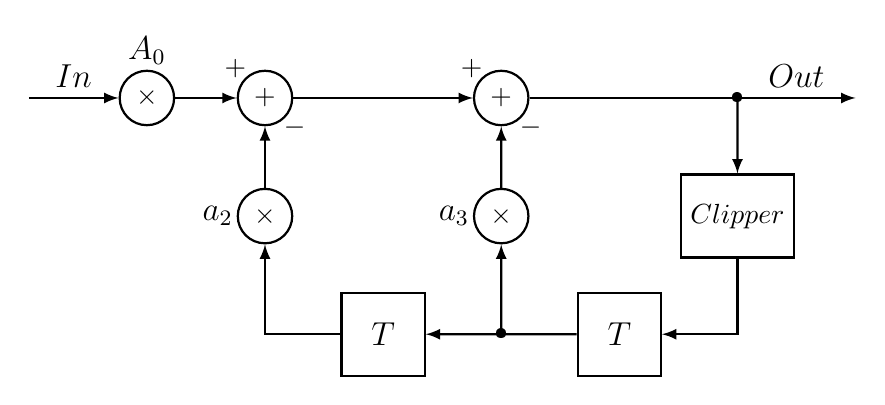
\begin{tikzpicture}[auto, thick, node distance=0.6cm, >=latex, scale = 0.75]

	\draw
	% Drawing the blocks of first filter 
	node at (-2,0) [prod] (p1) {\product} node[above of =p1]{\large$A_0$}
	node at (0,0)[sum] (s1) {$+$} node at ( -.5,.5){$+$}  node at ( .5,-.5){$-$}
	node at (4,0)[sum] (s2) {$+$} node at ( 3.5,.5){$+$}  node at ( 4.5,-.5){$-$}
	
	node at (4,-2) [prod] (p3) {\product} node[left of =p3]{\large$a_3$}
	node at (2,-4) [delay] (d1) {\delay} %node[above of = p2] {\large$$}
	node at (8,-2) [delay] (d3) {$Clipper$}
	node at (6,-4) [delay] (d2) {\delay} 
	node at (0,-2) [prod] (p2) {\product} node[left of =p2]{\large$a_2$};
	
	\draw[->](-4,0) -- node {\large$In$}(p1);
	\draw[->](p1) -- (s1);
	\draw[->](s1) --  (s2);
	\draw[-](s2) --  (8,0);
	\draw[->](8,0) -- node {\large$Out$}(10,0);
	\draw[->](8,0) --  (d3);
	\draw[->](d3) |-  (d2);
	\draw[->](d2) --  (d1);
	\draw[->](d1) -| (p2);
	\draw[->](p2) --  (s1);
	\draw[->](4,-4) --  (p3);
	\draw[->](p3) --  (s2);

	\draw
	node at (8,0) {\textbullet}
	node at (4,-4){\textbullet};
	
\end{tikzpicture}
\\Figure 1.1 Rossum's nonlinear resonator
\end{center}
 
 A Matlab implementation of Rossum's nonlinear resonator is given in following block.
 \begin{lstlisting}
function y = nlreson(fc, bw, limit, x)
% function y = nlreson(fc, bw, limit, x)
% Authors: Yangang Cao
% Parameters:
% fc = center frequency (in Hz)
% bw = bandwidth of resonance (in Hz)
% limit = saturation level
% x = input signal

fs = 44100;  % Sampling rate
R = 1 - pi*(bw/fs);  % Calculate pole radius
costheta = ((1+(R*R))/(2*R))*cos(2*pi*(fc/fs)); % Cosine of pole angle
a1 = -2*R*costheta;  % Calculate first filter coefficient
a2 = R*R;  % Calculate second filter coefficient
A0 = (1 - R*R)*sin(2*pi*(fc/fs)); % Scale factor
y = zeros(size(x));  % Allocate memory for output signal
w1 = 0; w2 = 0;  % Initialize state variables (unit delays)
y(1) = A0*x(1);  % The first input sample goes right through
w0 = y(1);  % Input to the saturating nonlinearity
for n = 2:length(x);  % Process the rest of input samples
	if y(n-1) > limit
		w0 = limit;  % Saturate above limit
	elseif y(n-1) < -limit
		w0 = -limit;  % Saturate below limit
	else 
		w0 = y(n-1);
	end  % Otherwise do nothing
	w2 = w1;  % Update the second state variable
	w1 = w0;  % Update the first state variable
	y(n) = A0*x(n) - a1*w1 - a2*w2;  % Compute filter output
end
 \end{lstlisting}
\subsection{Linear and nonlinear digital models of the Moog ladder filter}
Next we dicuss a well-known analog filter originally proposed by Robert Moog for his synthesizer designs. The filter consists of four one-pole filters in cascade and a global negative feedback loop.Stilson and Smith have considered various methods of converting the Moog ladder filter into a corresponding digital filter, an unit delay was inserted into the feedback loop to solve delay-free path from input to output, see figure 1.2.
\begin{center}
	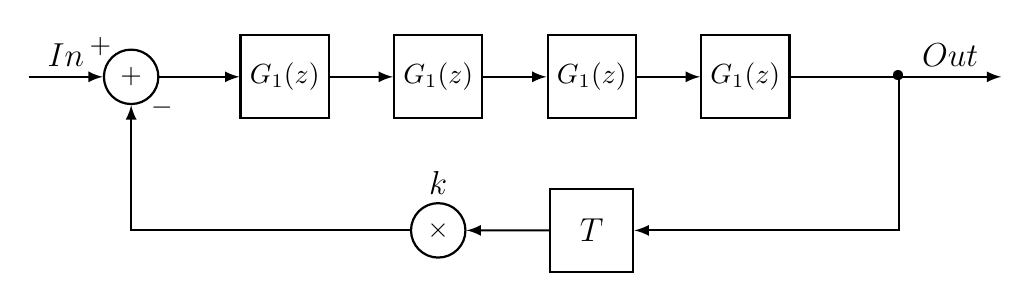
\begin{tikzpicture}[auto, thick, node distance=0.6cm, >=latex, scale = 0.65]
	
	\draw
	node at (0,0) [sum] (s1) {$+$} node at ( -.6,.6){$+$}  node at ( .6,-.6){$-$}
	node at (3,0) [delay] (d1) {$G_1(z)$}
	node at (6,0) [delay] (d2) {$G_1(z)$}
	node at (9,0) [delay] (d3) {$G_1(z)$}
	node at (12,0) [delay] (d4) {$G_1(z)$}
	node at (6,-3) [prod] (p1) {\product} node [above of = p1] {\large$k$}
	node at (9,-3) [delay] (d5) {\delay};

	\draw[->](-2,0) -- node {\large$In$}(s1);
	\draw[->](s1) -- (d1);
	\draw[->](d1) -- (d2);
	\draw[->](d2)--(d3);
	\draw[->](d3)--(d4);
	\draw[-](d4)--(15,0);
	\draw[->](15,0)--node{\large$Out$}(17,0);
	\draw[->](15,0)|-(d5);
	\draw[->](d5)--(p1);
	\draw[->](p1)-|(s1);
	
	
	\draw
	node at (15,0) {\textbullet};
	
	\end{tikzpicture}
	\\Figure 1.2 Digital Moog filter structure
\end{center}

Another complication in the discretization of the Moog filter is that the constant-Q control of the cornor frequency is lost, Stilson and Smith have found a usrful compromise first-order filter that has largely independent control of the Q value with cornor frequency:
\[
G_1(z) = \frac{1+p}{1.3}\frac{1+0.3z^{-1}}{1+pz^{-1}},
\]
where $0\leqslant p\leqslant1$ is the pole location. It can be determined conveniently from the normalized cut-off frequency $f_c$ (in Hz),
\[
p = \frac{f_c}{f_S}.
\]

Other researchers have considered the nonlinear behavior of the Moog filter. Huovilainen first derived a physically correct nonlinear model for the Moog filter, including the nonlinear behavior of all transistors involved, see figure 1.3.
\begin{center}
	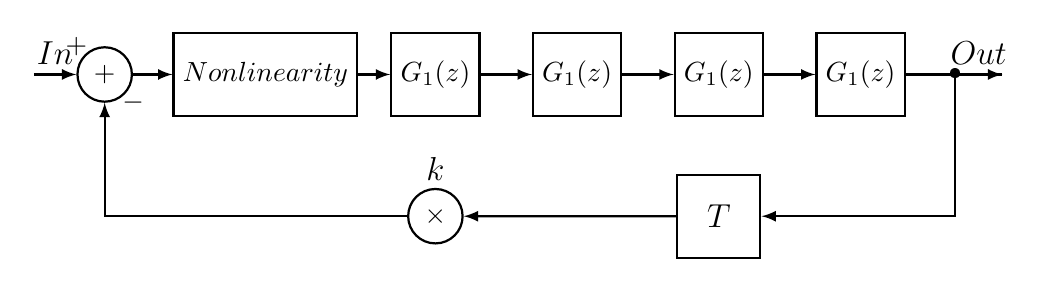
\begin{tikzpicture}[auto, thick, node distance=0.6cm, >=latex, scale = 0.6]
	
	\draw
	node at (-4,0) [sum] (s1) {$+$} node at ( -4.6,.6){$+$}  node at (-3.4,-.6){$-$}
	node at (-0.6,0) [delay] (d6) {$Nonlinearity$}
	node at (3,0) [delay] (d1) {$G_1(z)$}
	node at (6,0) [delay] (d2) {$G_1(z)$}
	node at (9,0) [delay] (d3) {$G_1(z)$}
	node at (12,0) [delay] (d4) {$G_1(z)$}
	node at (3,-3) [prod] (p1) {\product} node [above of = p1] {\large$k$}
	node at (9,-3) [delay] (d5) {\delay};
	
	\draw[->](-5.5,0) -- node {\large$In$}(s1);
	\draw[->](s1) -- (d6);
	\draw[->](d6) -- (d1);
	\draw[->](d1) -- (d2);
	\draw[->](d2)--(d3);
	\draw[->](d3)--(d4);
	\draw[-](d4)--(15,0);
	\draw[->](14,0)--node{\large$Out$}(15,0);
	\draw[->](14,0)|-(d5);
	\draw[->](d5)--(p1);
	\draw[->](p1)-|(s1);
	
	\draw
	node at (14,0) {\textbullet};
	
	\end{tikzpicture}
	\\Figure 1.3 Simplified nonlinear Moog filter structure
\end{center}

A Matlab implementation of the simplified nonlinear Moog filter is given in following block.
\begin{lstlisting}
function [out,out2,in2,g,h0,h1] = moogvcf(in,fc,res)
% function [out,out2,in2,g,h0,h1] = moogvcf(in,fc,res)
% Authors: Yangang Cao
% Parameters:
% in = input signal
% fc= cutoff frequency (Hz)
% res = resonance (0...1 or larger for self-oscillation)

fs = 44100;  % Input and output sampling rate
fs2 = 2*fs;  % Internal sampling rate
% Two times oversampled input signal:
in = in(:); in2 = zeros(1,2*length(in)); in2(1:2:end) = in; 
h = fir1(10,0.5); in2 = filter(h,1,in2);  % Anti-imaging filter
Gcomp = 0.5;  % Compensation of passband gain
g = 2*pi*fc/fs2;  % IIR feedback coefficient at fs2
Gres = res;  % Direct mapping (no table or polynomial)
h0 = g/1.3; h1 = g*0.3/1.3; % FIR part with gain g
w = [0 0 0 0 0]; % Five state variables
wold = [0 0 0 0 0];  % Previous states (unit delays)
out = zeros(size(in)); out2 = zeros(size(in2));
for n = 1:length(in2),
	u = in2(n) - 4*Gres*(wold(5) - Gcomp*in2(n));  % Input and feedback
	w(1) = tanh(u);  % Saturating nonlinearity
	w(2) = h0*w(1) + h1*wold(1) + (1-g)*wold(2);  % First IIR1
	w(3) = h0*w(2) + h1*wold(2) + (1-g)*wold(3);  % Second IIR1
	w(4) = h0*w(3) + h1*wold(3) + (1-g)*wold(4);  % Third IIR1
	w(5) = h0*w(4) + h1*wold(4) + (1-g)*wold(5);  % Fourth IIR1
	out2(n) = w(5);  % Filter output
	wold = w;  % Data move (unit delays)
end
out2 = filter(h,1,out2);  % Antialiasing filter at fs2
out = out2(1:2:end);  % Decimation by factor 2 (return to original fs)
\end{lstlisting}
\subsection{Wah-wah Filter}
The wah-wah effect is produced mostly by foot-controlled signal processors containing a bandpass filter with variable center frenquency and a small bandwith. Moving the pedal back and forth changes the bandpass center frequency. Typically this resonance is second-order, this section will describe digitization of the "CryBaby" wah-wah filter.

Based on the measured shape of the amplitude response and knowledge that the bandpass is second-order, the transfer function can be presumed to be of the form:

\[
H(s) = g\frac{s-\xi}{(\frac{s}{\omega_r})^2 + \frac{2}{Q}(\frac{s}{\omega_r})+1},
\]
where $g$ is an overall gain factor, $\xi$ is a real zero at or near dc(the other being at infinity), $\omega_r$ is the pole resonance frequency, and $Q$ is quality factor of the resonator. The measurements reveal that $\omega_r$, $Q$ and $g$ all vary significantly with pedal angle $\theta$, good choices for these functions are as shown in following Matlab code.
\begin{lstlisting}
function [g,fr,Q] = wahcontrols(wah)
% function [g,fr,Q] = wahcontrols(wah)
% Authors: Yangang Cao
% Parameter: wah = wah-pedal-angle normalized to lie between 0 and 1

g  = 0.1*4^wah;       % overall gain for second-order s-plane transfer funct.
fr = 450*2^(2.3*wah); % resonance frequency (Hz) for the same transfer funct.
Q  = 2^(2*(1-wah)+1); % resonance quality factor for the same transfer funct.
\end{lstlisting}

Closed-form expressions for digital filter coefficients in terms of $(Q, fr, g)$ based on $z = e^{st} \approx 1 + sT$ (low-frequency resonance assumed) yield the code shown in following code.
\begin{lstlisting}
% Authors:Yangang Cao
% A = wahdig(fr,Q,fs)
% 
% Parameters:
% fr = resonance frequency (Hz)
% Q  = resonance quality factor
% fs = sampling frequency (Hz)
%
% Returned:
% A = [1 a1 a2] = digital filter transfer-function denominator poly

frn = fr/fs;
R = 1 - Pi*frn/Q; % pole radius
theta = 2*Pi*frn; % pole angle
a1 = -2.0*R*cos(theta); % biquad coeff
a2 = R*R;               % biquad coeff

\end{lstlisting}
\end{document}
